% !TEX program = xelatex
% Compile with: xelatex -interaction=nonstopmode heron_final_presentation.tex
\documentclass[aspectratio=169,11pt]{beamer}

% ---------- Language and fonts ----------
\usepackage{fontspec}
\setsansfont{DejaVu Sans}
\setmainfont{DejaVu Serif}
\setmonofont{DejaVu Sans Mono}
\usepackage{polyglossia}
\setmainlanguage{english}

% ---------- Packages ----------
\usepackage{graphicx}
\usepackage{booktabs}
\usepackage{tabularx}
\usepackage{array}
\usepackage{xcolor}
\usepackage{ragged2e}
\usepackage{tikz}
\usetikzlibrary{arrows.meta,positioning,fit,calc,shapes.geometric}
\usepackage[most]{tcolorbox}
\usepackage{etoolbox}
\usepackage{amsmath}
\usepackage{amssymb}

% ---------- HERON-inspired colors ----------
\definecolor{HeronBlue}{HTML}{1497CF}
\definecolor{HeronDark}{HTML}{4F5156}
\definecolor{HeronLight}{HTML}{EAF6FC}
\definecolor{HeronSoft}{HTML}{F7FAFC}
\definecolor{HeronGreen}{HTML}{2E8B57}
\definecolor{HeronOrange}{HTML}{D8902F}
\definecolor{HeronRed}{HTML}{C4514A}
\definecolor{HeronGray}{HTML}{D9DEE2}

% ---------- Beamer styling ----------
\setbeamertemplate{navigation symbols}{}
\setbeamertemplate{blocks}[rounded][shadow=false]
\setbeamertemplate{itemize items}[circle]
\setbeamercolor{title}{fg=HeronDark}
\setbeamercolor{frametitle}{fg=HeronDark}
\setbeamercolor{normal text}{fg=HeronDark,bg=white}
\setbeamercolor{structure}{fg=HeronBlue}
\setbeamerfont{title}{series=\bfseries,size=\LARGE}
\setbeamerfont{frametitle}{series=\bfseries,size=\large}
\setbeamerfont{subtitle}{size=\large}
\setbeamerfont{author}{size=\normalsize}
\setbeamerfont{caption}{size=\scriptsize}
\setbeamersize{text margin left=0.55cm,text margin right=0.55cm}
\setlength{\tabcolsep}{4pt}

\setbeamertemplate{frametitle}{%
  \vspace{0.12cm}%
  {\color{HeronBlue}\rule[-0.12em]{3pt}{1.0em}}\hspace{0.45em}\insertframetitle\par%
  \vspace{-0.15cm}%
  {\color{HeronBlue}\rule{\linewidth}{0.7pt}}%
}

% ---------- Metadata ----------
\newcommand{\StudentName}{Marina Fragkouli}
\newcommand{\StudentEmail}{marina.frag3@gmail.com}
\newcommand{\GitHub}{https://github.com/marina-frag/crowd\_aware\_ws}
\newcommand{\InternshipTopic}{Crowd-Aware Front-Following for Assistive Mobile Robots}
\newcommand{\SupervisorNames}{Georgios Moustris, Andreas Vatistas}
\newcommand{\MeetingLabel}{Final Presentation}
\newcommand{\MeetingDate}{25 November 2026}

\title[HERON Internship]{Final Internship Presentation}
\subtitle{\InternshipTopic}
\author{\StudentName}
\institute{HERON -- Hellenic Robotics Center of Excellence}
\date{\MeetingLabel\;|\;\MeetingDate}

\setbeamertemplate{footline}{%
  \leavevmode%
  \hbox{%
    \begin{beamercolorbox}[wd=.80\paperwidth,ht=2.5ex,dp=1ex,leftskip=1.2em]{author in head/foot}%
      \textcolor{HeronDark}{\insertshorttitle}\hspace{0.7em}\textcolor{HeronBlue}{|}\hspace{0.7em}\MeetingLabel
    \end{beamercolorbox}%
    \begin{beamercolorbox}[wd=.20\paperwidth,ht=2.5ex,dp=1ex,rightskip=1.2em plus1fil]{date in head/foot}%
      \hfill\textcolor{HeronDark}{\insertframenumber/\inserttotalframenumber}
    \end{beamercolorbox}%
  }%
}

% ---------- Helpers ----------
\newcolumntype{Y}{>{\RaggedRight\arraybackslash}X}
\newcolumntype{L}[1]{>{\RaggedRight\arraybackslash}p{#1}}
\newcolumntype{C}[1]{>{\Centering\arraybackslash}p{#1}}

\newtcolorbox{statusbox}[2][]{%
  enhanced,
  colback=#2!6,
  colframe=#2,
  boxrule=0.7pt,
  arc=2mm,
  left=2mm,right=2mm,top=1.2mm,bottom=1.2mm,
  #1
}

\newcommand{\takeaway}[1]{%
  \begin{statusbox}{HeronBlue}
    \footnotesize\textbf{Takeaway:} #1
  \end{statusbox}
}

\newcommand{\done}{\textcolor{HeronGreen}{\textbf{done}}}
\newcommand{\running}{\textcolor{HeronOrange}{\textbf{running}}}
\newcommand{\planned}{\textcolor{HeronDark}{planned}}

% ---------- Graphics helpers ----------
\tikzset{
  chip/.style={rounded corners=2pt,inner sep=2.5pt,font=\tiny\bfseries,text=white},
  chev/.style={signal,signal to=east,signal from=west,minimum height=0.62cm,inner xsep=6pt,
    font=\scriptsize,text=white},
  demoicon/.style={line width=0.9pt}}
\usetikzlibrary{shapes.symbols}
\newcommand{\badge}[2]{\tikz[baseline=-0.6ex]\node[circle,fill=#1,text=white,inner sep=1.2pt,
  minimum size=1.15em,font=\scriptsize\bfseries]{#2};}

% Speaker-notes slides: \shownotesfalse hides them, \shownotestrue prints them
\newif\ifshownotes
\shownotesfalse

\begin{document}

% ---------- Title ----------
\begin{frame}[plain]
  \vspace{0.2cm}
  \begin{columns}[T,totalwidth=\textwidth]
    \begin{column}{0.28\textwidth}
      \IfFileExists{heron_logo.png}{%
        
\includegraphics[width=0.88\linewidth]{heron_logo.png}%
      }{%
        {\Large\bfseries\textcolor{HeronBlue}{HERON}}%
      }
    \end{column}
    \begin{column}{0.70\textwidth}
      \raggedleft
      {\Large\bfseries HERON}\par
      {\small Hellenic Robotics Center of Excellence}
    \end{column}
  \end{columns}
  \vfill
  \begin{center}
    {\usebeamerfont{title}\textcolor{HeronDark}{\inserttitle}}\par\vspace{0.25cm}
    {\usebeamerfont{subtitle}\textcolor{HeronBlue}{\insertsubtitle}}\par\vspace{0.45cm}
    {\large \StudentName}\par
    {\small \StudentEmail}\par\vspace{0.25cm}
    {\small \GitHub}\par\vspace{0.25cm}
    {\small Supervisors: \SupervisorNames}\par\vspace{0.25cm}
    {\bfseries \MeetingLabel}\quad {\MeetingDate}
  \end{center}
  \vfill
\end{frame}

% ---------- Motivation ----------
\begin{frame}{Motivation}
  \begin{center}
    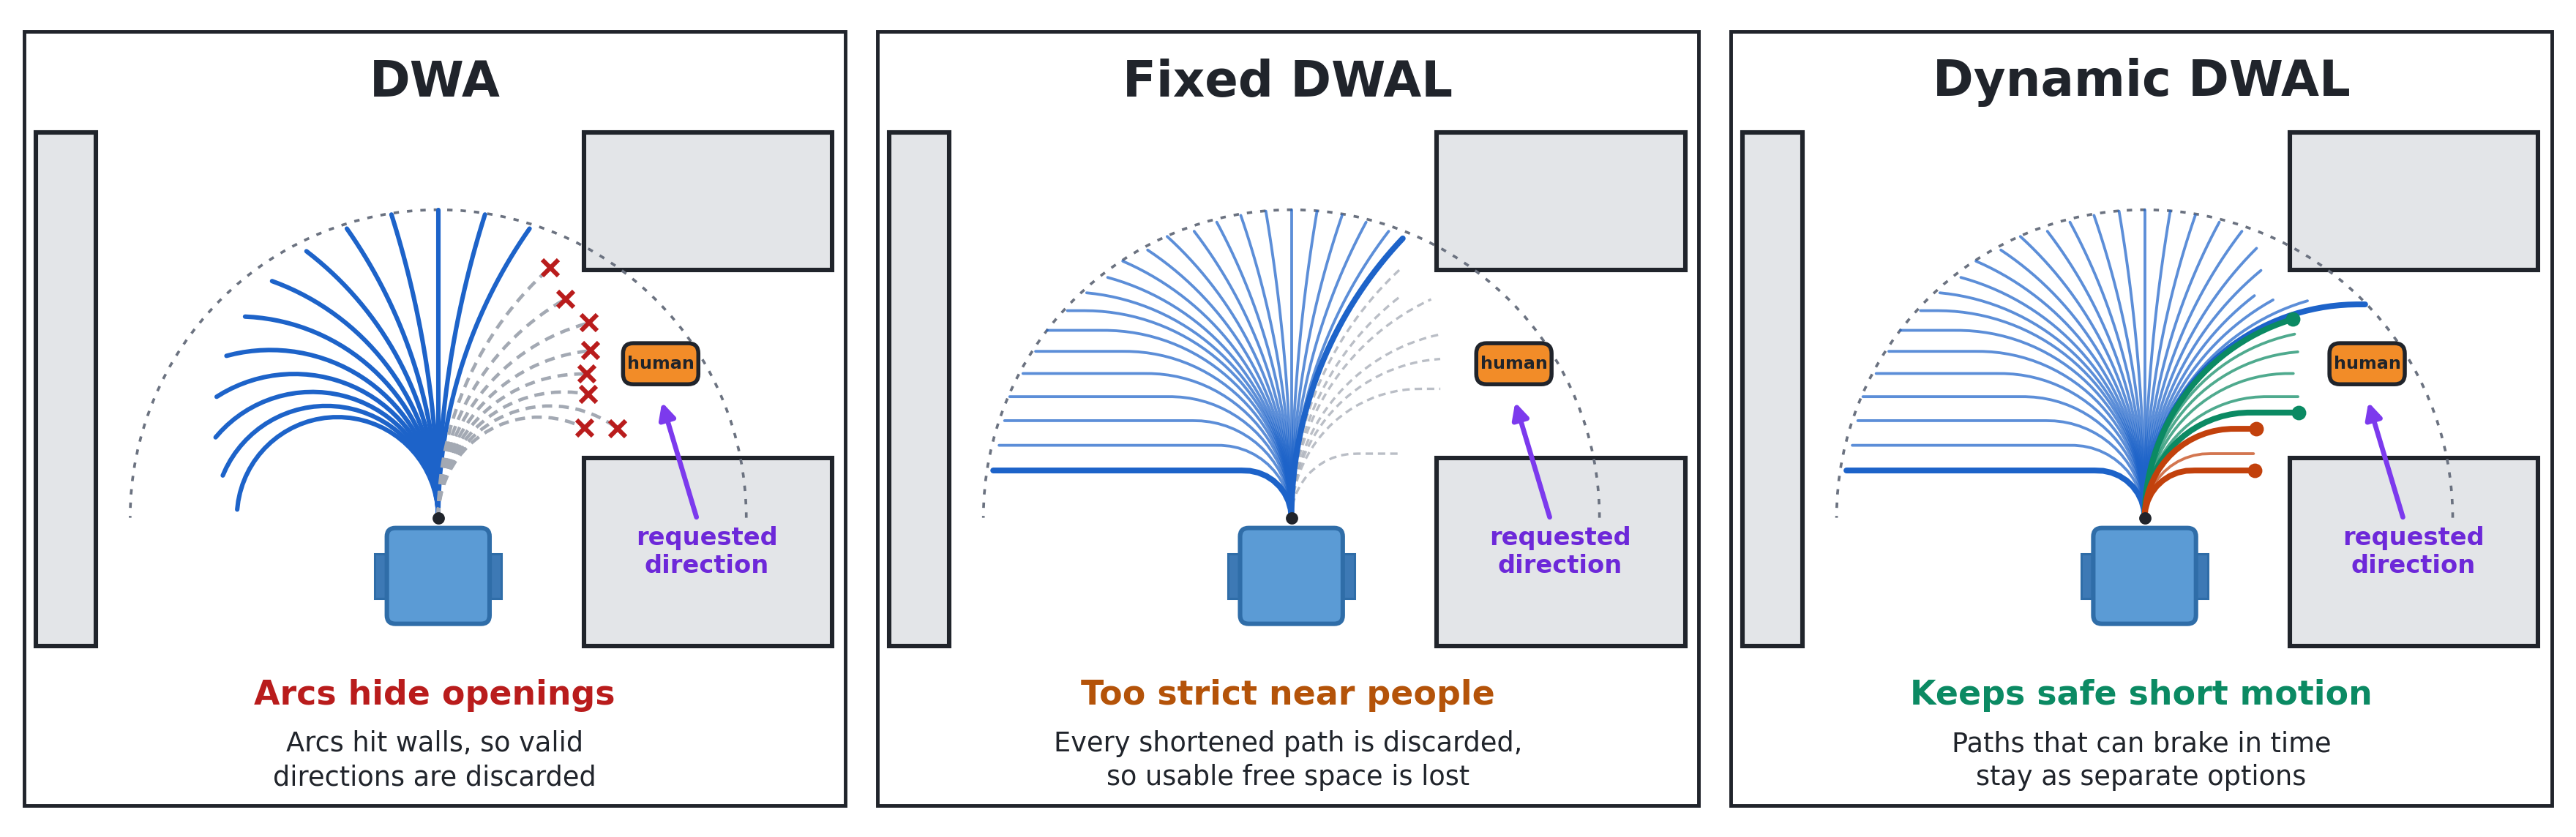
\includegraphics[width=0.82\linewidth]{images/motivation_dwa_dwal.png}\par
    \vspace{0.05cm}
    {\scriptsize\textcolor{HeronBlue}{Figure:} DWA vs Fixed DWAL vs Dynamic DWAL (schematic scene, computed paths)}\par
  \end{center}
  \vspace{0.12cm}
  \begin{statusbox}{HeronBlue}
    \footnotesize\textbf{Contribution:}
    A Nav2-compatible, crowd-aware local pipeline.
  \end{statusbox}
  \vspace{0.15cm}
\end{frame}

\ifshownotes
\begin{frame}{Motivation Speaker Notes}
  Αρχικά να δούμε λίγο το κίνητρο. Ξεκινώντας με το παραδοσιακό NAV2
controller dwa


\textbf{DWA $\rightarrow$ DWAL}
\begin{itemize}
  \item O DWA παράγει τόξα σταθερής καμπυλότητας, που δεν ταιριάζουν στην εύρεση ανοιγμάτων, δηλαδή διακριτών διαδρομών.
  \item Τα τόξα χτυπούν στους τοίχους και έτσι απορρίπτουν έγκυρες κατευθύνσεις κίνησης.
  \item Η απάντηση ο DWAL ο οποίος χρησιμοποιεί αντί για τόξα arclines αλλά
όπως και ο DWA απορρίπτει κάθε path που κόβεται από εμπόδιο.
\end{itemize}

\vspace{0.2cm}
Ποιο είναι το πρόβλημα με τον DWAL:
\textbf{Fixed DWAL $\rightarrow$ Dynamic DWAL}
\begin{itemize}
  \item Σε πειράματα με το πραγματικό ρομπότ σε πλήθος παρατηρήθηκαν εκτεταμένα διαστήματα όπου ζητούνταν κίνηση, υπήρχε χώρος και το ρομπότ έμενε ακίνητο.
  \item \textbf{Υπόθεση:} η απόρριψη κάθε path που συναντά εμπόδιο πριν τον ορίζοντα είναι υπερβολικά αυστηρή σε πυκνό πλήθος.
\end{itemize}
\end{frame}
\fi

% ---------- Definitions ----------
\tikzset{robotdot/.style={fill=HeronDark}, freepath/.style={HeronGreen,line width=1.2pt},
  defnote/.style={font=\scriptsize,text=HeronDark,inner sep=1pt},
  deftitle/.style={font=\footnotesize\bfseries,text=HeronDark,anchor=north},
  defcell/.style={draw=HeronGray,rounded corners=3pt,fill=HeronSoft}}

\begin{frame}{Relevant Definitions}
  \centering
  \resizebox{!}{5.25cm}{\begin{tikzpicture}[x=1cm,y=1cm]
    % six cells of 4.7 x 2.85 cm: columns at x = 0, 4.95, 9.9; rows at y = 0, -3.05
    \foreach \cx in {0,4.95,9.9} \foreach \cy in {0,-3.05}
      \draw[defcell] (\cx,\cy) rectangle ++(4.7,-2.85);
    \node[deftitle] at (2.35,-0.08)  {Path (arc-line)};
    \node[deftitle] at (7.30,-0.08)  {Free length $L$, radius $r$};
    \node[deftitle] at (12.25,-0.08) {Horizon};
    \node[deftitle] at (2.35,-3.13)  {Cluster};
    \node[deftitle] at (7.30,-3.13)  {Motion choice};
    \node[deftitle] at (12.25,-3.13) {Path end vs robot front};

    % --- Path: arc up to 90 deg, then the tangent line (metres, k = 0, 1, 2 1/m, horizon 1.8 m) ---
    \begin{scope}[shift={(1.5,-2.5)},scale=1.15]
      \draw[HeronGray!80!black,line width=0.8pt] (0,0) -- (1.8,0);
      \draw[HeronGray!80!black,line width=0.8pt] (0,0) arc[start angle=-90,end angle=0,radius=1] -- ++(0,0.229);
      \draw[freepath] (0,0) arc[start angle=-90,end angle=0,radius=0.5] coordinate (k) -- ++(0,1.015);
      \fill[HeronOrange] (k) circle (2.2pt);
      \node[defnote,text=HeronGreen,left] at (0.3,0.35) {arc ≤ 90°};
      \node[defnote,text=HeronGreen,left] at (0.48,1.1) {line};
      \node[defnote,text=HeronGray!60!black,above] at (1.55,0) {k = 0};
      \node[defnote,text=HeronGray!60!black,right] at (1.0,1.0) {k = 1};
      \node[defnote,text=HeronGreen,right] at (0.5,1.35) {k = 2};
      \fill[robotdot] (0,0) circle (2.5pt);
    \end{scope}

    % --- Free length L vs free radius r ---
    \begin{scope}[shift={(6.2,-2.6)},scale=0.95]
      \draw[freepath] (0,0) arc[start angle=-90,end angle=0,radius=0.8] -- ++(0,0.5) coordinate (e);
      \fill[HeronOrange] ($(e)+(0,0.3)$) circle (0.2);
      \draw[HeronDark,dashed,line width=0.8pt] (0,0) -- (e);
      \fill[HeronGreen] (e) circle (2.2pt);
      \node[defnote,text=HeronGreen,right] at (0.85,0.55) {$L$: along the path};
      \node[defnote,left] at (0.3,0.75) {$r$: straight};
      \fill[robotdot] (0,0) circle (2.5pt);
    \end{scope}

    % --- Horizon (robot at (10.6,-1.6)) ---
    \begin{scope}[shift={(10.75,-1.65)},scale=0.55]
      \foreach \a in {-40,-20,0,20,40} \draw[HeronGray!80!black,line width=0.8pt] (0,0) -- (\a:2.6);
      \draw[HeronBlue,dashed,line width=1pt] (-48:2.6) arc[start angle=-48,end angle=48,radius=2.6];
      \node[defnote,text=HeronBlue,right] at (2.65,0) {1.8 m};
      \fill[robotdot] (0,0) circle (2.5pt);
    \end{scope}

    % --- Cluster (robot at (0.8,-4.75)) ---
    \begin{scope}[shift={(0.8,-4.75)},scale=0.6]
      \foreach \a in {20,30,40,50} \draw[HeronBlue,line width=0.9pt] (0,0) -- (\a:2.2);
      \foreach \a in {-20,-30,-40,-50} \draw[HeronGreen,line width=0.9pt] (0,0) -- (\a:2.2);
      \foreach \a in {-8,0,8} \draw[HeronOrange,line width=0.9pt] (0,0) -- (\a:1.3);
      \fill[HeronRed!70] (1.6,0) circle (0.25);
      \node[defnote,text=HeronBlue,right] at (35:2.3) {left};
      \node[defnote,text=HeronGreen,right] at (-35:2.3) {right};
      \node[defnote,text=HeronOrange,right] at (1.9,0) {towards};
      \fill[robotdot] (0,0) circle (2.5pt);
    \end{scope}

    % --- Motion choice (robot at (5.6,-4.7)) ---
    \begin{scope}[shift={(5.6,-4.7)},scale=0.62]
      \draw[HeronBlue,dashed,line width=0.8pt] (15:3.0) arc[start angle=15,end angle=45,radius=3.0];
      \draw[freepath,-{Latex[length=1.6mm]}] (0,0) -- (30:3.0);
      \node[defnote,text=HeronGreen,above left] at (30:1.7) {pass};
      \draw[HeronRed,line width=1.2pt] (0,0) -- (-12:1.5);
      \draw[HeronRed,line width=1.6pt] ($(-12:1.5)+(78:0.2)$) -- ($(-12:1.5)+(-102:0.2)$);
      \fill[HeronOrange] (-12:2.05) circle (0.25);
      \node[defnote,text=HeronRed,below] at (0.7,-0.3) {brake};
      \fill[robotdot] (0,0) circle (2.5pt);
    \end{scope}

    % --- Path end vs robot front (base_link at (10.4,-4.75)) ---
    \begin{scope}[shift={(10.25,-4.75)},x=1.6cm,y=1.6cm]
      \fill[HeronBlue!25] (0,-0.2) rectangle (0.97,0.2);
      \draw[HeronBlue,line width=0.8pt] (0,-0.2) rectangle (0.97,0.2);
      \fill[HeronDark] (0.103,0) circle (1.5pt);
      \node[defnote,below] at (0.3,-0.2) {\texttt{base\_link}};
      \fill[HeronOrange] (2.18,-0.27) rectangle (2.32,0.27);
      \draw[freepath] (0.103,0) -- (1.21,0);
      \fill[HeronGreen] (1.21,0) circle (1.6pt);
      \node[defnote,text=HeronGreen,above] at (0.66,0.2) {path};
      \draw[HeronGray!75!black,dashed,line width=0.9pt] (1.21,0) -- (2.18,0);
      \draw[{Latex[length=1.2mm]}-{Latex[length=1.2mm]}] (1.21,-0.4) -- (2.18,-0.4);
      \node[defnote,below] at (1.7,-0.4) {0.885 m body};
    \end{scope}
  \end{tikzpicture}}
  \vspace{0.05cm}
  \takeaway{A cluster is a motion option the user can choose: left of, right of, or towards an obstacle.}
\end{frame}

\ifshownotes
\begin{frame}{Relevant Definitions Speaker Notes}
\footnotesize
\begin{itemize}\setlength{\itemsep}{1pt}
  \item \textbf{Path:} κινηματικά εφικτό arc-line, τόξο έως $90^\circ$ και μετά εφαπτόμενη ευθεία, μέσα στο dynamic window συγκεκριμένη καμπυλότητα και συγκεκριμένη δειγματοληψία($\Delta t = 0.2$ s, καμπυλότητα έως $\pm 4$).
  \item \textbf{Free length $L$:} απόσταση πάνω στο path μέχρι το footprint να ακουμπήσει εμπόδιο ή να τελειώσει το path.
  \item \textbf{Free radius $r$:} ευθεία απόσταση από το ρομπότ ως το τέλος του path.
  \item \textbf{Horizon:} τα paths αξιολογούνται έως $1.8$ m.
  \item \textbf{Cluster:}  Ένα cluster είναι ένα σύνολο κινηματικά εφικτών, ελεύθερων paths που
αντιστοιχούν στην ίδια επιλογή κίνησης
 Όταν υπάρχει εμπόδιο μπροστά, οι επιλογές είναι τρεις:
προς το εμπόδιο (με φρενάρισμα πριν από αυτό), δεξιά του, αριστερά του.
  \item \textbf{Motion choice:} Κάθε path χαρακτηρίζεται ως pass (φτάνει τον ορίζοντα) ή brake (σταματά σε εμπόδιο). Χρησιμοποιούνται μόνο στην αξιολόγηση, ως ground truth για τον χαρακτηρισμό των clusters σχετικά με το αν κάνουν overclustering, underclustering και την σταθερότητά τους.
\end{itemize}
\end{frame}
\fi

% ---------- Fixed vs Dynamic ----------
\begin{frame}{Fixed vs Dynamic pipeline}
  \footnotesize
  \renewcommand{\arraystretch}{1.0}
  \begin{tabularx}{\textwidth}{@{}L{2.8cm}YY@{}}
    \toprule
    \textbf{Stage} & \textbf{Fixed DWAL} & \textbf{Dynamic DWAL}\\
    \midrule
    Path acceptance & Free beyond a fixed radius $R$ ($1.2$ or $1.8$ m) & Free for at least the \textbf{braking distance} at the current speed\\
    Clustering & Split at gaps between free paths & Gaps \textbf{and} free-length discontinuities $|\Delta L| > \tau$\\
    Correspondence & Upstream cluster matching & \textbf{Frame-to-frame ID tracking}\\
    Velocity & Near / far level with speed hysteresis & Paths without forward speed removed by a \textbf{braking model}; otherwise rotate only\\
    \bottomrule
  \end{tabularx}

  \vspace{0.1cm}
  \begin{columns}[c,totalwidth=\textwidth]
    \begin{column}{0.62\textwidth}
      \centering\footnotesize
      $S_{\mathrm{req}}(v) = vT + \dfrac{v^2}{2a} + m$\par
      {\scriptsize $T=0.4$ s,\; $a=0.5$ m/s$^2$,\; $m=0.05$ m \;$\Rightarrow$\; $0.26$ m at $0.3$ m/s}\par
      \vspace{0.12cm}
      $S_{\mathrm{req}}(v) \le L \;\Leftrightarrow\; v \le v_{\max}(L) = \sqrt{a^2T^2 + 2a\,(L-m)} - aT$
    \end{column}
    \begin{column}{0.36\textwidth}
      \centering
      \begin{tikzpicture}[x=2.3cm,y=0.75cm,font=\tiny]
        \draw[HeronDark!60,-{Latex[length=1.2mm]}] (0,0) -- (1.08,0) node[below left] {$v$ [m/s]};
        \draw[HeronDark!60,-{Latex[length=1.2mm]}] (0,0) -- (0,1.6) node[left] {[m]};
        \fill[HeronGreen!15] (0,0) rectangle (0.689,0.8);
        \draw[HeronBlue,line width=1.1pt,domain=0:1,samples=40] plot (\x,{0.4*\x+\x*\x+0.05});
        \node[HeronBlue,right] at (0.98,1.45) {$S_{\mathrm{req}}$};
        \draw[HeronOrange,line width=1pt] (0,0.8) -- (1.02,0.8) node[right] {$L$};
        \draw[HeronDark,dashed] (0.689,0.8) -- (0.689,0);
        \fill[HeronDark] (0.689,0.8) circle (1.4pt);
        \node[below] at (0.689,0) {$v_{\max}$};
        \node[HeronGreen!70!black] at (0.3,0.55) {admissible};
      \end{tikzpicture}
    \end{column}
  \end{columns}
  \vspace{0.05cm}
  \takeaway{Shorter paths become usable, so clustering can no longer rely on free gaps alone.}
\end{frame}

\ifshownotes
\begin{frame}{Fixed vs Dynamic pipeline Speaker Notes}
  Υπενθυμίζουμε ότι ουσιαστικά εμείς θέλουμε να βελτιώσουμε τον DWAL και για να το πετύχουμε αυτό αλλάζουμε τα εξής σημεία:
\begin{itemize}
  \item \textbf{Μεταβλητό μήκος:} αντί να ζητάμε πάντα ελεύθερο το ίδιο R, ζητάμε τουλάχιστον όσο χρειάζεται για να φρενάρει το ρομπότ με την τωρινή ταχύτητα.
  \item \textbf{Clustering:} αφού κρατάμε και κοντά paths, το clustering του fixed δεν αρκεί, γιατί θα ένωνε σε ένα cluster paths που περνούν με paths που σταματούν.
  \item \textbf{Correspondence:} το ίδιο cluster πρέπει να κρατά το ίδιο ID από frame σε frame, αλλιώς η πρόθεση του χρήστη δεν μένει σταθερή. Αυτό σχετίζεται και με τα πρότζεκτ του Θανάση και του Κώστα.
  \item \textbf{Ταχύτητα:} η κίνηση περιορίζεται από το μοντέλο πέδησης, άρα το ρομπότ προχωρά μόνο όσο προλαβαίνει να σταματήσει. Στην διαφάνεια βλέπουμε και μια ανισωση η οποία σχετίζεται με το μοντέλο της πέδησης και συμφωνα με την επιλυση τως ως προς u οριζεται η εννοια του admissible velocity που ειναι μια εννοια που υπήρχε στο DWA αλλά όχι στον DWAL
\end{itemize}
\end{frame}
\fi

% ---------- Clustering ----------
\begin{frame}{Clustering}
  \begin{columns}[T,totalwidth=\textwidth]
    \begin{column}{0.47\textwidth}
      \footnotesize
      \textbf{\textcolor{HeronBlue}{What a good clustering does}}
      \begin{itemize}\setlength{\itemsep}{3pt}
        \item \textbf{Underclustering as Homogeneity violation ($U$):} each cluster contains one motion choice.
        \item \textbf{Overclustering as Completeness violation ($O$):} each motion choice stays in one cluster.
        \item \textbf{Stability ($S$):} ID switches per minute.
      \end{itemize}
      \vspace{0.1cm}
      \[
        \mathrm{Loss} = \frac{U}{0.395} + \frac{O}{0.028} + \frac{S}{0.833}
      \]
      {\scriptsize Denominators frozen at the step 2 peaks.\par}
    \end{column}
    \begin{column}{0.50\textwidth}
      \footnotesize
      \textbf{\textcolor{HeronBlue}{Split rules compared (step 3.1)}}\par\vspace{0.12cm}
      \renewcommand{\arraystretch}{1.25}
      \begin{tabularx}{\linewidth}{@{}L{1.85cm}YL{1.45cm}@{}}
        \toprule
        \textbf{Method} & \textbf{Rule} & \textbf{Values}\\
        \midrule
        Length jump & $|\Delta L| > \tau$ & $\tau$: 0.1, 0.2, 0.3\\
        Change-point & Piecewise-linear fit of $r$, penalty $\beta$ per cut & $\beta$: 0.05, 0.2, 0.4\\
        DBSCAN & Endpoint density, radius $\varepsilon$, minPts 3 & $\varepsilon$: 0.1, 0.15\\
        \bottomrule
      \end{tabularx}
    \end{column}
  \end{columns}
  \vspace{0.2cm}
  \takeaway{Selection: same runs as $\tau=0.3$, 0 collisions, at least as many goals, then the lowest Loss.}
\end{frame}

\ifshownotes
\begin{frame}{Clustering Speaker Notes}
\begin{itemize}
  \item \textbf{Underclustering:} μετριέται ως παραβίαση homogeneity: κάθε cluster πρέπει να έχει paths μίας μόνο επιλογής. Παραβίαση είναι ένα cluster με pass και brake, αλλά και ένα cluster με pass 1 και pass 2, γιατί γεφυρώνει ένα εμπόδιο.
  \item \textbf{Overclustering:} μετριέται ως παραβίαση completeness: κάθε κατηγορία πρέπει να βρίσκεται σε ένα cluster
  \item \textbf{Stability:} μετριέται ως ID switches ανά λεπτό.
  \item Τα ονόματα homogeneity και completeness είναι από Rosenberg \& Hirschberg (2007). Εμείς μετράμε ποσοστό παραβιάσεων.
  \item Τα παραπάνω κανονικοοποιούνται και χρησιμοποιούνται για να ορίσουμε ένα Loss σύμφωνα με το οποίο συγκρίνουμε τις μεθόδους clustering.
  \item Οι μέθοδοι που συγκρίναμε ήταν τρεις: length jump, change-point και DBSCAN. Κάθε μέθοδος χρειάστηκε fine tune ως προς μία παράμετρο.
  \item Τα αποτελέσματα των συγκρίσεων φαίνονται σε επόμενη διαφάνεια
\end{itemize}
\end{frame}
\fi

% ---------- Pipeline ----------
\begin{frame}{Pipeline}
  \centering
  \vspace{0.25cm}
  \resizebox{0.97\linewidth}{!}{%
  \begin{tikzpicture}[
    node distance=0.42cm and 0.48cm,
    box/.style={draw=HeronBlue,rounded corners=2pt,fill=white,minimum width=2.9cm,minimum height=1.05cm,align=center,font=\scriptsize},
    changed/.style={box,draw=HeronOrange,fill=HeronOrange!12,line width=1.1pt},
    safety/.style={box,draw=HeronGreen,fill=HeronGreen!8},
    arrow/.style={-{Latex[length=2mm]},HeronDark,semithick}
  ]
    \node[box] (cost) {Local costmap\\+ iWalk footprint};
    \node[changed,right=of cost] (gen) {\textbf{Path generator}\\variable free length};
    \node[changed,right=of gen] (clu) {\textbf{Clustering}\\split + ID tracking};
    \node[box,right=of clu] (intent) {Intent estimator\\selects a cluster};
    \node[changed,below=0.75cm of intent] (shared) {\textbf{Shared controller}\\path, $v$, $\omega$};
    \node[safety,left=of shared] (smooth) {Velocity\\smoother};
    \node[safety,left=of smooth] (monitor) {Collision\\monitor};
    \node[safety,left=of monitor] (watch) {Watchdog\\$\rightarrow$ robot base};
    \draw[arrow] (cost) -- (gen);
    \draw[arrow] (gen) -- (clu);
    \draw[arrow] (clu) -- (intent);
    \draw[arrow] (intent) -- (shared);
    \draw[arrow] (shared) -- (smooth);
    \draw[arrow] (smooth) -- (monitor);
    \draw[arrow] (monitor) -- (watch);
    \draw[arrow,HeronOrange,dashed] (shared.north west) -- node[left,font=\tiny,align=right] {braking\\requirement} (clu.south east);
  \end{tikzpicture}%
  }

  \vspace{0.3cm}
  {\scriptsize
    \textcolor{HeronOrange}{\rule{0.28cm}{0.18cm}} modified in this work \qquad
    \textcolor{HeronBlue}{\rule{0.28cm}{0.18cm}} upstream, unchanged \qquad
    \textcolor{HeronGreen}{\rule{0.28cm}{0.18cm}} safety and command layers\par}
  \vspace{0.2cm}
  \raggedright
  \takeaway{The safety layers stay outside the planner, so the method changes options, not the final safety stack.}
\end{frame}

\ifshownotes
\begin{frame}{Pipeline Speaker Notes}
Οι παραπάνω διαφορές καθορίζουν το pipeline στο οποίο καταλήξαμε.
\begin{itemize}
  \item Ο generator δίνει τα paths με το ελεύθερο μήκος τους.
  \item Το clustering χωρίζει τις επιλογές και κρατά σταθερά IDs.
  \item Ο intent estimator μένει ίδιος και επιλέγει cluster από την εντολή του χρήστη.
  \item Ο shared controller βγάζει $v$ και $\omega$ και στέλνει πίσω την απαίτηση φρεναρίσματος στο clustering.
  \item Velocity smoother, collision monitor του NAV2 και custom watchdog εφαρμόζονται και στις δύο μεθόδους.
\end{itemize}
\end{frame}
\fi

% ---------- Hypotheses and metrics ----------
\begin{frame}{Hypothesis and Metrics}
  \footnotesize
  \renewcommand{\arraystretch}{1.3}
  \begin{tabularx}{\textwidth}{@{}L{1.0cm}YL{5.2cm}@{}}
    \toprule
    & \textbf{Hypothesis} & \textbf{Metric}\\
    \midrule
    \textbf{H1} & Variable length reduces standstill while motion is requested & Standstill time [s], tracking $-$ fixed\\
    \textbf{H2} & Length-jump clustering gives clusters consistent with the definition and a low Loss & Homogeneity, completeness, Loss\\
    \textbf{H3} & Tracking correspondence keeps cluster IDs more stable than the existing greedy matching & ID switches/min, offline replay on the same clusters\\
    \textbf{H4} & The path selected by the whole pipeline is natural: close to the teleoperator's path in SCAND & $|\varphi^{*}-\varphi_{\mathrm{true}}|$ at 1.8\,m, ADE/FDE vs.\ a user-only baseline\\
    \bottomrule
  \end{tabularx}

  \vspace{0.2cm}
  \begin{statusbox}{HeronBlue}
    \scriptsize\textbf{Statistics:} paired runs (same scenario, path, seed), Wilcoxon signed-rank, rank-biserial $r$, bootstrap 95\% CI, Holm over H1 and H3.\\[2pt]
    \textbf{Revised H1 rule (post-hoc):} Holm $p<0.05$, CI of the \textbf{mean} difference excludes 0, 0 collisions, personal-zone time not significantly worse. Obstacle distance is always reported as a trade-off.
  \end{statusbox}
\end{frame}

\ifshownotes
\begin{frame}{Hypothesis and Metrics Speaker Notes}
Υποθέτουμε τα εξής:
\begin{itemize}
  \item \textbf{H1:} το μεταβλητό μήκος μειώνει τον χρόνο ακινησίας όταν ο χρήστης ζητά κίνηση.
  \item \textbf{H2:} το clustering με length jump φτιάχνει clusters συμβατά με τον ορισμό (μία επιλογή κίνησης ανά cluster, χωρίς να σπάει μια επιλογή σε κομμάτια) και με χαμηλό Loss.
  \item \textbf{H3:} το tracking correspondence κρατά τα IDs πιο σταθερά από το υπάρχον greedy matching, δηλαδή δίνει λιγότερα ID switches.
  \item \textbf{H4:} το path που επιλέγει όλο το pipeline είναι «φυσικό», δηλαδή κοντά στη διαδρομή του χειριστή στο SCAND (teleoperated robots σε κοινωνικά περιβάλλοντα).
\end{itemize}
\end{frame}
\fi

% ---------- Protocol ----------
\begin{frame}{Evaluation Protocol}
  \begin{columns}[T,totalwidth=\textwidth]
    \begin{column}{0.60\textwidth}
      \scriptsize
      \renewcommand{\arraystretch}{1.28}
      \begin{tabularx}{\linewidth}{@{}L{0.55cm}YL{1.15cm}@{}}
        \toprule
        \textbf{Step} & \textbf{Purpose} & \textbf{Status}\\
        \midrule
        1 & Path deviation, no obstacles & \done\\
        2 & Select $\tau$ (180 runs) & \done\\
        3 & Fixed vs tracking: 13 conditions, seeds 1--10, 260 runs & \done\\
        3.1 & Tune $\tau$, $\beta$, $\varepsilon$ with and without walls, 480 runs & \done\\
        4 & Compare methods on SCAND recordings & \planned\\
        5 & Apply the decision rules & in progress\\
        6 & Broad confirmation: 50 seeds, 900 runs & \planned\\
        \bottomrule
      \end{tabularx}
    \end{column}
    \begin{column}{0.38\textwidth}
      \centering
      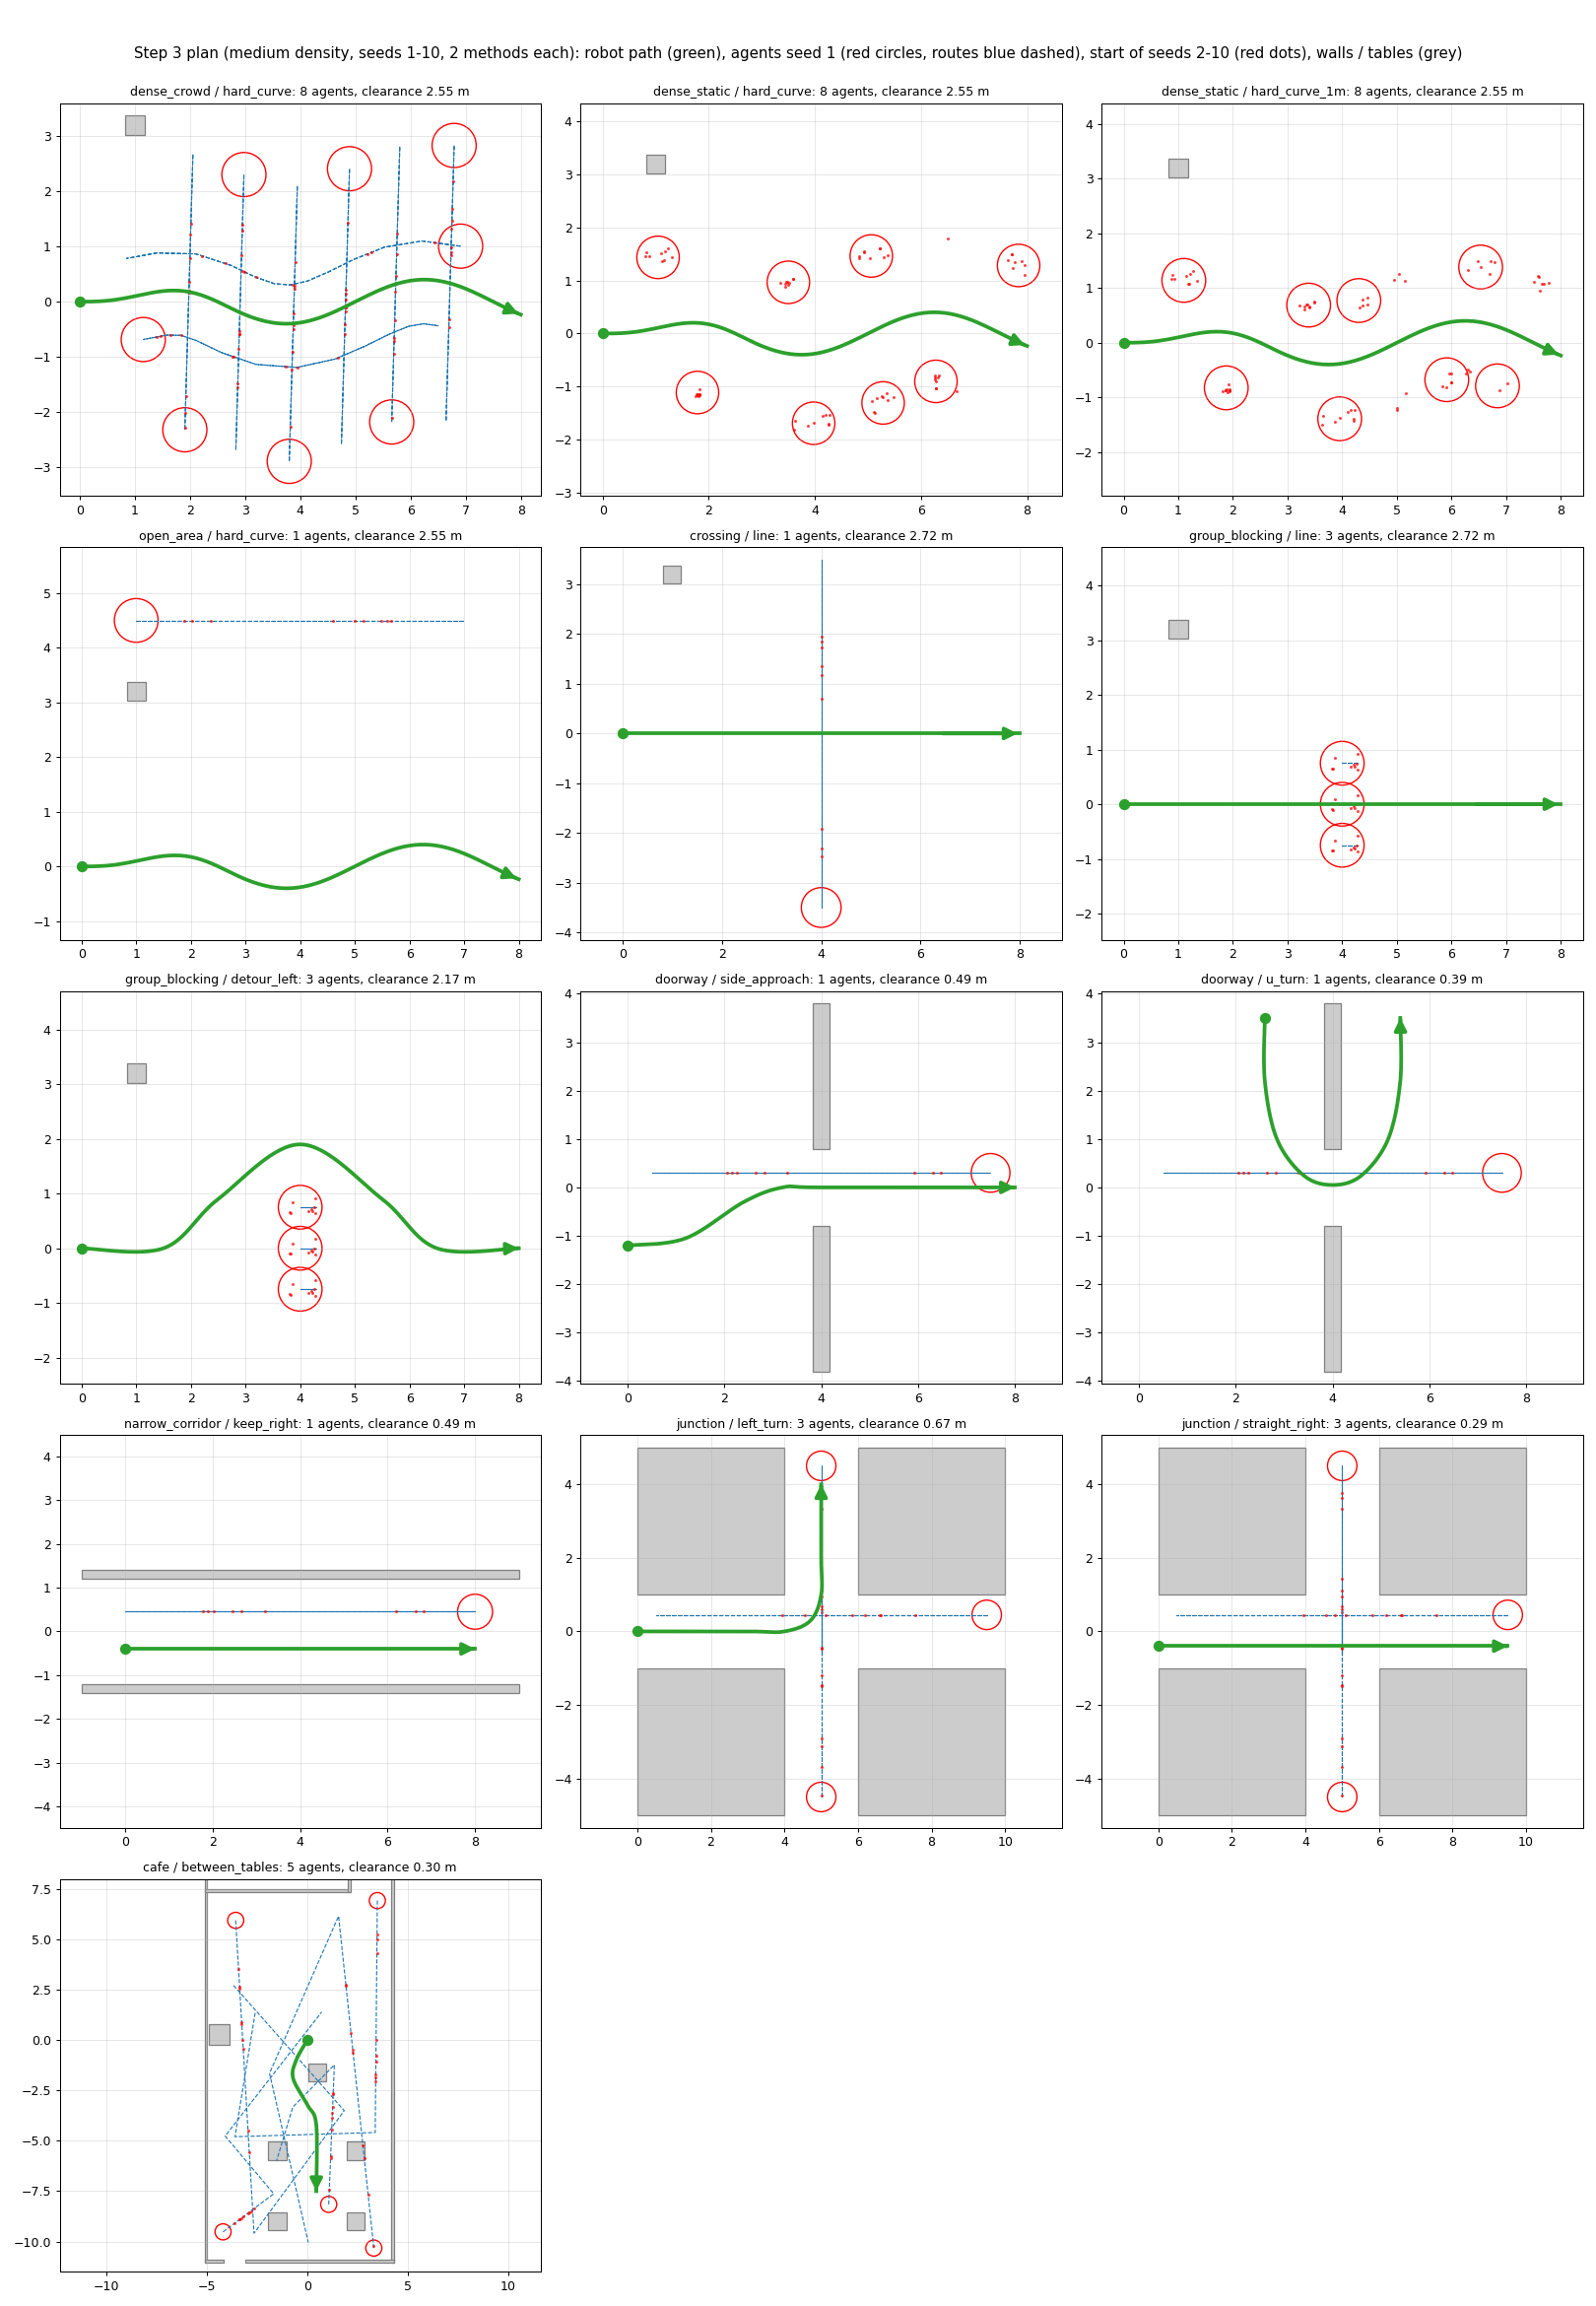
\includegraphics[height=0.72\textheight]{images/step3_plan.png}\par
      {\tiny Step 3: 13 scenario conditions\par}
    \end{column}
  \end{columns}
\end{frame}

\ifshownotes
\begin{frame}{Evaluation Protocol Speaker Notes}
\begin{itemize}
  \item Πάμε να δούμε τώρα το προτόκολλο αξιολόγησης που ελέγχει τόσο το συνολικό αποτέλεσμα του pipeline όσο συγκρίνει και τις επιμέρους μεθόδους. Τα αποτελέσματα ανά βήμα:
  \item Το βήμα 1 δείχνει ότι χωρίς εμπόδια fixed και tracking πράγματι ακολουθούν την ίδια διαδρομή αυτό είναι σαν baseline.
  \item Το βήμα 2 κάνει fine tune στην παράματρο τ της μεθόδου μας και το βήμα 3 συγκρίνει τις μεθόδους με αυτό.
  \item Το βήμα 3.1 προστέθηκε για να δοκιμάσουμε και tuning και σε άλλα σενάρια πχ με τοίχους και τις επιπλέον μεθόδους clustering.
  \item Τα βήματα 4 και 6 δεν έχουν τρέξει ακόμα.
  \item Eνώ δεξιά βλέπουμε τα usecases-σενάρια που χρησιμοποιήθηκαν στο βήμα 3.
\end{itemize}
\end{frame}
\fi

% ---------- Results ----------
\begin{frame}{Results per step: Steps 1 and 2}
  \begin{columns}[T,totalwidth=\textwidth]
    \begin{column}{0.48\textwidth}
      \footnotesize
      \textbf{\textcolor{HeronBlue}{Step 1: path deviation}}\par\vspace{0.12cm}
      \scriptsize
      \begin{tabular}{@{}lcc@{}}
        \toprule
        Path & Fixed max [m] & Tracking max [m]\\
        \midrule
        line & 0.001 & 0.001\\
        s\_curve & 0.017 & 0.016\\
        hard\_curve & 0.091 & 0.092\\
        \bottomrule
      \end{tabular}\par
      \vspace{0.18cm}
      \begin{tikzpicture}[x=26cm,y=0.34cm,font=\tiny]
        \foreach \n/\f/\k/\y in {line/0.001/0.001/0, s\_curve/0.017/0.016/-1, hard\_curve/0.091/0.092/-2} {
          \node[anchor=east,text=HeronDark] at (-0.004,\y) {\n};
          \fill[HeronGray!90!black] (0,\y+0.05) rectangle (\f,\y+0.38);
          \fill[HeronGreen] (0,\y-0.05) rectangle (\k,\y-0.38);
        }
        \draw[HeronDark!60] (0,0.6) -- (0,-2.6);
        \draw[HeronDark!60] (0,-2.6) -- (0.1,-2.6);
        \foreach \v in {0,0.05,0.1} \node[below,text=HeronDark!80] at (\v,-2.6) {\v};
        \node[below,text=HeronDark!80] at (0.05,-3.15) {max deviation [m]};
        \fill[HeronGray!90!black] (0.068,0.35) rectangle ++(0.004,0.3); \node[right] at (0.072,0.5) {Fixed};
        \fill[HeronGreen] (0.068,-0.25) rectangle ++(0.004,0.3); \node[right] at (0.072,-0.1) {Tracking};
      \end{tikzpicture}\hfill
      % the three desired paths, to scale (8 m long; prepare_scene.py build_path)
      \begin{tikzpicture}[x=0.25cm,y=0.25cm,font=\tiny]
        \draw[HeronBlue,line width=0.9pt,-{Latex[length=1.1mm]}] (0,3.9) -- (8,3.9);
        \draw[HeronBlue,line width=0.9pt,-{Latex[length=1.1mm]}] plot[domain=0:8,samples=61,smooth] (\x,{1.7+1.5*(\x/8-sin(deg(2*pi*\x/8))/(2*pi))});
        \draw[HeronBlue,line width=0.9pt,-{Latex[length=1.1mm]}] plot[domain=0:8,samples=81,smooth] (\x,{0.4*sin(deg(2*pi*\x/5))*min(\x/3,1)^2*(3-2*min(\x/3,1))});
        \foreach \y in {3.9,1.7,0} \fill[HeronDark] (0,\y) circle (0.14);
        \node[anchor=south west,inner sep=1pt,text=HeronDark] at (0,3.95) {line};
        \node[anchor=south east,inner sep=1pt,text=HeronDark] at (8,1.7) {s\_curve};
        \node[anchor=south west,inner sep=1pt,text=HeronDark] at (0,0.45) {hard\_curve};
        \node[anchor=north,inner sep=1pt,text=HeronDark!80] at (4,-0.5) {8\,m, to scale};
      \end{tikzpicture}\par
      \vspace{0.1cm}
      \footnotesize Without obstacles the two methods follow the same path.
    \end{column}
    \begin{column}{0.48\textwidth}
      \footnotesize
      \textbf{\textcolor{HeronBlue}{Step 2: selecting $\tau$}}\par\vspace{0.12cm}
      \scriptsize
      \begin{tabular}{@{}ccccc@{}}
        \toprule
        $\tau$ & $U$ & $O$ & $S$ & Loss\\
        \midrule
        0.1 & 0.037 & 0.028 & 0.33 & 1.493\\
        0.2 & 0.086 & 0.007 & 0.47 & 1.014\\
        \textbf{0.3} & \textbf{0.133} & \textbf{0.003} & \textbf{0.40} & \textbf{0.919}\\
        \bottomrule
      \end{tabular}\par
      \vspace{0.18cm}
      \begin{tikzpicture}[x=1.15cm,y=0.8cm,font=\tiny]
        \foreach \t/\l/\c [count=\i] in {0.1/1.493/HeronGray!90!black, 0.2/1.014/HeronGray!90!black, 0.3/0.919/HeronBlue} {
          \fill[\c] (\i-0.3,0) rectangle (\i+0.3,\l);
          \node[above,text=HeronDark] at (\i,\l) {\l};
          \node[below,text=HeronDark] at (\i,0) {$\tau = \t$};
        }
        \draw[HeronDark!60] (0.5,0) -- (3.5,0);
        \node[rotate=90,text=HeronDark!80] at (0.3,0.8) {Loss};
        \node[chip,fill=HeronGreen] at (3,1.5) {lowest};
      \end{tikzpicture}\par
      \vspace{0.1cm}
      \footnotesize $\tau = 0.3$ has the lowest Loss.
      \par{\tiny dense\_crowd, dense\_static $\times$ 3 densities, line, 5 seeds (30 runs per $\tau$). $\tau = 0.5,\,0.7,\,1.0$: rejected by the definition filter.\par}
    \end{column}
  \end{columns}
  \vspace{0.1cm}
  \takeaway{The control chain is validated, and $\tau = 0.3$ is the reference value for the next steps.}
\end{frame}

\ifshownotes
\begin{frame}{Results per step: Steps 1 2 Speaker Notes}
\begin{itemize}
  \item Εδώ βλέπουμε τα αποτελέσματα των βημάτων 1 και 2.
  \item Στο βήμα 1 βλέπουμε ότι χωρίς εμπόδια οι δύο μέθοδοι ακολουθούν την ίδια διαδρομή δοκιμάσαμε ευθεία γραμμή και δύο καμπύλες. Όπως βλεπουμε κάθε διαδρομή είναι αυξανόμενης δυσκολίας.
  \item Στο βήμα 2 τεστάραμε σε σενάρια dense\_crowd και dense\_static, με τρεις πυκνότητες (sparse, medium, dense), ευθεία διαδρομή και 5 seeds (101--105), δηλαδή 30 runs ανά τιμή του τ, για να αιτιολογήσουμε την επιλογή της παραμέτρου τ. Όπως βλέπουμε η τιμή τ=0.3 δίνει το χαμηλότερο Loss.
  \item Τρέξαμε και τ = 0.5, 0.7 και 1.0. Απορρίφθηκαν από το φίλτρο του ορισμού (χειρότερο κελί πάνω από 0.25), γι' αυτό δεν είναι στον πίνακα. Όλες οι τιμές είχαν 0 συγκρούσεις και έφτασαν στον στόχο.
\end{itemize}

\end{frame}
\fi

\begin{frame}{Results per step: Step 3}
  \begin{columns}[T,totalwidth=\textwidth]
    \begin{column}{0.53\textwidth}
      \footnotesize
      \textbf{H1: variable length reduces standstill} {\scriptsize (130 pairs)}
      \begin{itemize}\setlength{\itemsep}{2pt}
        \item Mean standstill: \textbf{18.3 s $\rightarrow$ 6.9 s}
        \item Difference $-11.4$ s, 95\% CI $[-15.6,\,-7.5]$
        \item Holm $p < 0.0001$
        \item Goal reached: \textbf{112/130} vs \textbf{56/130}
        \item \textbf{0 collisions} with both methods
        \item Personal-zone time: no significant change
        \item \textbf{Trade-off:} median obstacle distance $-4.7$ cm
      \end{itemize}
      \vspace{0.05cm}
      {\scriptsize
      \textbf{H2} (descriptive): lowest Loss in step 2; 6th of 8 with walls (step 3.1)\\
      \textbf{H3:} not confirmed, Holm $p = 0.36$ (105/130 pairs tied)\\
      \textbf{H4:} not tested yet (SCAND, step 4)\par}
    \end{column}
    \begin{column}{0.45\textwidth}
      \centering
      \begin{tikzpicture}[x=0.052cm,y=0.42cm]
        \draw[HeronDark] (0,0) -- (62,0);
        \foreach \v/\l in {0/0,20/20,40/40,60/60} {
          \draw[HeronGray] (\v,0) -- (\v,5.0);
          \node[font=\tiny,below] at (\v,0) {\l};
        }
        \node[font=\tiny] at (31,-1.05) {median standstill [s]};
        \foreach \y/\n/\f/\t in {4.3/junction left/58.6/0.2,3.3/junction straight/57.0/0.1,2.3/doorway side/31.5/0.2,1.3/corridor/28.4/0.1,0.4/dense crowd/6.6/0.1} {
          \fill[HeronGray!85!black] (0,\y) rectangle (\f,\y+0.28);
          \fill[HeronBlue] (0,\y-0.3) rectangle (\t+0.6,\y-0.02);
          \node[font=\tiny,left] at (0,\y) {\n};
        }
        \fill[HeronGray!85!black] (8,5.45) rectangle (11,5.75);
        \node[font=\tiny,right] at (11,5.6) {fixed};
        \fill[HeronBlue] (30,5.45) rectangle (33,5.75);
        \node[font=\tiny,right] at (33,5.6) {tracking};
      \end{tikzpicture}
    \end{column}
  \end{columns}
  \vspace{0.05cm}

\end{frame}

\ifshownotes
\begin{frame}{Results per step: Steps 3 Speaker Notes}
\footnotesize
\begin{itemize}
  \item Για το βήμα 3 τώρα είδαμε πριν λίγες διαφανειες ποια σενάρια χρησιμοποιήσαμε.
  \item Γενικά το κέρδος φαίνεται κυρίως σε junction, corridor και πυκνό πλήθος. Στις ανοιχτές σκηνές οι μέθοδοι είναι ίδιες.
  \item Συγκεκριμένα σχετικά με την υπόθεση H1
  \begin{itemize}
    \item Το tracking μειώνει τον χρόνο ακινησίας κατά 11.4 s, με 95\% CI [-15.6, -7.5] και Holm p < 0.0001.
    \item Το tracking φτάνει στον στόχο στα διπλάσια runs (112 έναντι 56), χωρίς σύγκρουση.
    \item Το κόστος είναι ότι περνά πιο κοντά σε εμπόδια, κατά $4.7$ cm στη διάμεσο
  \end{itemize}
  \item Για τις υπόλοιπες υποθέσεις:
  \begin{itemize}
    \item H2 δεν είναι κύριο τεστ στο βήμα 3, γιατί fixed και tracking βάζουν σε cluster διαφορετικά paths. Στο βήμα 2 το τ = 0.3 περνά το φίλτρο του ορισμού με το χαμηλότερο Loss. Με τοίχους (βήμα 3.1) είναι 6ο στα 8.
    \item H3 δεν επιβεβαιώνεται: τα ID switches είναι σπάνια και στους δύο τρόπους, 105 από τα 130 ζεύγη είναι ισοπαλία, Holm p = 0.36.
    \item H4 δεν έχει ελεγχθεί ακόμα. Θα κριθεί στο SCAND (βήμα 4).
  \end{itemize}
\end{itemize}

\end{frame}
\fi

\begin{frame}{Results per step: Step 3.1}
  \begin{statusbox}{HeronGreen}
    \footnotesize\textbf{We keep $\tau = 0.3$:} the only value that reaches 59/60 goals. No new closed-loop runs needed.
  \end{statusbox}
  \vspace{0.05cm}
  \scriptsize
  \renewcommand{\arraystretch}{1.08}
  \begin{tabularx}{\textwidth}{@{}Ycccccc@{}}
    \toprule
    \textbf{Value} & \textbf{Collisions} & \textbf{Goals /60} & $U$ & $O$ & $S$ & \textbf{Loss}\\
    \midrule
    \textbf{$\boldsymbol{\tau = 0.3}$ (selected)} & \textbf{0} & \textbf{59} & \textbf{0.190} & \textbf{0.003} & \textbf{0.45} & \textbf{1.127}\\
    $\varepsilon = 0.15$ & 0 & 58 & 0.108 & 0.008 & 0.35 & 0.992\\
    $\tau = 0.2$ & 0 & 57 & 0.144 & 0.006 & 0.33 & 0.989\\
    $\beta = 0.2$ & 0 & 57 & 0.146 & 0.007 & 0.40 & 1.112\\
    $\beta = 0.4$ & 0 & 56 & 0.181 & 0.005 & 0.28 & 0.986\\
    $\beta = 0.05$ & 0 & 55 & 0.084 & 0.013 & 0.30 & 1.037\\
    $\varepsilon = 0.1$ & 0 & 55 & 0.068 & 0.014 & 0.42 & 1.189\\
    $\tau = 0.1$ & 0 & 55 & 0.068 & 0.035 & 0.40 & 1.922\\
    \bottomrule
  \end{tabularx}

  \vspace{0.08cm}
  {\scriptsize \textbf{Rule (locked before results):} same runs, 0 collisions, goals $\geq$ those of $\tau = 0.3$, then lowest Loss.\par
  \textbf{Not the best clustering:} five values have lower Loss, but each loses at least one goal.\par
  Obstacle distance for $\tau = 0.3$: mean minimum 0.41 m (60/60 runs).\par}
\end{frame}

\ifshownotes
\begin{frame}{Results per step Step 3.1 Speaker Notes}
\footnotesize
\begin{itemize}
  \item Το βήμα 2 έγινε χωρίς τοίχους, ενώ 6 από τις 13 συνθήκες του βήματος 3 έχουν τοίχους. Γι' αυτό στο 3.1 κάναμε ξανά tuning, με και χωρίς τοίχους, και δοκιμάσαμε δύο ακόμα κανόνες χωρισμού: DBSCAN στα endpoints (ε) και change-point στο r (β).
  \item Κάθε τιμή έτρεξε στα ίδια 60 runs: 6 κελιά χωρίς τοίχους και 6 συνθήκες με τοίχους, με 5 seeds (101--105). Σύνολο 480 runs.
  \item Ο κανόνας κλειδώθηκε πριν δούμε αποτελέσματα: 0 συγκρούσεις, τουλάχιστον τόσοι στόχοι όσοι με τ = 0.3, και μετά το μικρότερο Loss.
  \item Καμία τιμή δεν είχε σύγκρουση, αλλά μόνο το τ = 0.3 φτάνει τους 59/60 στόχους. Άρα μένει το τ = 0.3 και δεν χρειάζονται νέα closed-loop runs.
  \item Δεν είναι το καλύτερο clustering: πέντε τιμές έχουν μικρότερο Loss, και το τ = 0.3 έχει το υψηλότερο U. Η απόφαση είναι οριακή, γιατί το ε = 0.15 χάνει μόνο έναν στόχο.
  \item Η απόσταση από εμπόδια δεν είναι φίλτρο, απλώς την αναφέρουμε: για το τ = 0.3 η μέση ελάχιστη απόσταση είναι 0.41 m.
  \item Αν ρωτήσουν: διερευνητικά τρέξαμε και το ε = 0.15 σε closed-loop (130 runs). Έφτασε στον στόχο 117 έναντι 112 φορές, όλοι οι επιπλέον στόχοι στο doorway. Έτρεξε όμως με νεότερο Docker image, άρα η διαφορά δεν αποδίδεται με βεβαιότητα στο clustering και δεν αλλάζει το τ = 0.3.
\end{itemize}
\end{frame}
\fi

% ---------- Demo ----------
\begin{frame}{Demo}
  \begin{columns}[T,totalwidth=\textwidth]
    \begin{column}{0.325\textwidth}
      \begin{statusbox}[equal height group=demo]{HeronBlue}
        \centering
        \begin{tikzpicture}[scale=0.45,demoicon]
          \foreach \px/\py in {0.9/0.75,1.9/-0.75,2.9/0.75,3.6/-0.75} \fill[HeronOrange] (\px,\py) circle (0.22);
          \draw[HeronBlue,line width=1.4pt,-{Latex[length=2mm]}] plot[domain=0:4,samples=41,smooth] (\x,{0.35*sin(deg(2*pi*\x/2))});
          \fill[HeronDark] (0,0) circle (0.12);
        \end{tikzpicture}\par\vspace{2pt}
        \raggedright
        \badge{HeronBlue}{1}\;\footnotesize\textbf{Same frame, four split rules}\\[2pt]
        \scriptsize\texttt{dense\_static:hard\_curve}, seed 3\\
        Run ($\tau = 0.3$) vs.\ $\tau = 0.2$, $\varepsilon = 0.15$, $\beta = 0.2$
      \end{statusbox}
    \end{column}
    \begin{column}{0.325\textwidth}
      \begin{statusbox}[equal height group=demo]{HeronGreen}
        \centering
        \begin{tikzpicture}[scale=0.45,demoicon]
          \fill[HeronOrange] (1.2,0.75) circle (0.22); \fill[HeronOrange] (1.2,-0.75) circle (0.22);
          \fill[HeronOrange] (2.3,1.0) circle (0.22);
          \draw[HeronGreen,line width=1.4pt,-{Latex[length=2mm]}] (0,0) -- (1.6,0) arc[start angle=-90,end angle=0,radius=0.8] -- ++(0,0.5);
          \fill[HeronDark] (0,0) circle (0.12);
        \end{tikzpicture}\par\vspace{2pt}
        \raggedright
        \badge{HeronGreen}{2}\;\footnotesize\textbf{Where tracking helps}\\[2pt]
        \scriptsize\texttt{junction:left\_turn}, seed 6\\
        Fixed vs tracking, same agents
      \end{statusbox}
    \end{column}
    \begin{column}{0.325\textwidth}
      \begin{statusbox}[equal height group=demo]{HeronBlue}
        \centering
        \begin{tikzpicture}[x=0.5cm,y=0.26cm]
          \foreach \row/\segs in {2/{0/1/HeronGray,1/5/HeronOrange}, 1/{0/1/HeronGray,1/1.8/HeronGreen,1.8/4.2/HeronOrange,4.2/5/HeronGreen}, 0/{0/1/HeronGray,1/1.8/HeronGreen,1.8/4.2/HeronOrange,4.2/5/HeronGreen}}
            \foreach \a/\b/\c in \segs \fill[\c] (\a+0.04,\row*1.35) rectangle (\b-0.04,\row*1.35+1);
          \node[font=\tiny,anchor=east] at (0,3.2) {$\tau$}; \node[font=\tiny,anchor=east] at (0,1.85) {$\varepsilon$};
          \node[font=\tiny,anchor=east] at (0,0.5) {$\beta$};
        \end{tikzpicture}\par\vspace{2pt}
        \raggedright
        \badge{HeronBlue}{3}\;\footnotesize\textbf{Split rules between tables}\\[2pt]
        \scriptsize\texttt{cafe:between\_tables}, seed 3\\
        Same four rows, close to tables
      \end{statusbox}
    \end{column}
  \end{columns}
  \vspace{0.3cm}
  \begin{columns}[T,totalwidth=\textwidth]
    \begin{column}{0.49\textwidth}
      \footnotesize
      \textbf{How to read the replay}
      \begin{itemize}\setlength{\itemsep}{2pt}
        \item \textbf{Colored lines:} clusters, traced by \texttt{base\_link}.
        \item \textbf{Orange cylinders:} humans.
      \end{itemize}
    \end{column}
    \begin{column}{0.49\textwidth}
      \footnotesize
      \textbf{How to read the split-rule bars} (demos 1 and 3)\par\vspace{3pt}
      \scriptsize
      \tikz\fill[HeronGreen] (0,0) rectangle (0.35,0.2);\; pass \quad
      \tikz\fill[HeronGray] (0,0) rectangle (0.35,0.2);\; brake \quad
      \tikz\fill[HeronOrange] (0,0) rectangle (0.35,0.2);\; mixed (pass + brake)\par\vspace{2pt}
      Offline, open loop: the same scan through each rule. Top row: the clusters the run recorded.
    \end{column}
  \end{columns}
\end{frame}

\ifshownotes
\begin{frame}{Demo Speaker Notes}
\footnotesize
\begin{itemize}
  \item Τα demos είναι replay καταγεγραμμένων runs, άρα δεν εξαρτώνται από τη ζωντανή προσομοίωση.
  \item Demo 1 και 3: ίδιο scan, τέσσερις κανόνες χωρισμού. Η πάνω γραμμή είναι τα clusters που δημοσίευσε το run, οι άλλες τρεις είναι offline. Ένα καλό clustering δεν έχει πορτοκαλί (ανάμεικτο) cluster και δεν σπάει μια επιλογή σε πολλά κομμάτια.
  \item Demo 2: στο seed 6 το fixed μένει ακίνητο 58.7 s από τα 60 s ενώ ο χρήστης ζητά κίνηση και δεν φτάνει στον στόχο. Το tracking φτάνει στον στόχο σε 36.7 s, χωρίς σύγκρουση.
  \item Στο demo 2, μετά το πρώτο δευτερόλεπτο τα δύο ρομπότ βρίσκονται σε διαφορετικά σημεία, οπότε τα δύο panels δεν δείχνουν την ίδια στιγμή της σκηνής.
  \item Να υπάρχει εφεδρικό βίντεο σε περίπτωση που δεν ανοίξει το RViz.
\end{itemize}
\vspace{0.15cm}
\tiny
\texttt{TAU=0.2 EPS=0.15 BETA=0.2 bash scripts/demo\_side\_by\_side.sh cuts dense\_static:hard\_curve 3}\\[3pt]
\texttt{bash scripts/demo\_side\_by\_side.sh compare junction:left\_turn 6}\\[3pt]
\texttt{TAU=0.2 EPS=0.15 BETA=0.2 bash scripts/demo\_side\_by\_side.sh cuts cafe:between\_tables 3}
\end{frame}
\fi

% ---------- Constraints ----------
\begin{frame}{Constraints and next steps}
  \begin{columns}[T,totalwidth=\textwidth]
    \begin{column}{0.51\textwidth}
      \footnotesize
      \textbf{\textcolor{HeronRed}{Constraints}}
      \begin{itemize}\setlength{\itemsep}{3pt}
        \item Results are from \textbf{simulation}.
        \item The revised H1 rule is \textbf{post-hoc}.
        \item Doorway deadlock in 6 of 20 tracking runs.
        \item Tracking passes closer to obstacles.
        \item Semantics are off in these experiments.
        \item Paired runs do not share the exact start time of the first command.
      \end{itemize}
    \end{column}
    \begin{column}{0.46\textwidth}
      \footnotesize
      \textbf{\textcolor{HeronGreen}{Next steps}}
      \begin{itemize}\setlength{\itemsep}{3pt}
        \item Re-test $\beta$ and $\varepsilon$ on \textbf{new seeds}.
        \item Confirm H1 on \textbf{new seeds}.
        \item Evaluate on \textbf{SCAND} recordings.
        \item Find which code change fixed the doorway deadlock.
        \item Validate on the \textbf{real iWalk robot}.
      \end{itemize}
    \end{column}
  \end{columns}
  \vfill
  \begin{center}
    \begin{tikzpicture}[node distance=0.12cm]
      \node[chev,fill=HeronGreen] (a) {Simulation};
      \node[chev,fill=HeronBlue,right=of a] (b) {New seeds: confirm H1};
      \node[chev,fill=HeronBlue!75,right=of b] (c) {SCAND recordings};
      \node[chev,fill=HeronDark!80,right=of c] (d) {Real iWalk};
      \node[font=\tiny,text=HeronGreen,below=1pt of a] {done};
      \node[font=\tiny,text=HeronDark,below=1pt of b] {next};
      \node[font=\tiny,text=HeronDark,below=1pt of c] {planned};
      \node[font=\tiny,text=HeronDark,below=1pt of d] {planned};
    \end{tikzpicture}
  \end{center}
\end{frame}

\ifshownotes
\begin{frame}{Constraints and next steps Speaker Notes}
\begin{itemize}
  \item Το βασικό εύρημα είναι ότι το ρομπότ σταματά πολύ λιγότερο και φτάνει συχνότερα στον στόχο, χωρίς συγκρούσεις στην προσομοίωση.
  \item Για να γίνει ισχυρός ισχυρισμός χρειάζονται νέα seeds και πειράματα στο πραγματικό ρομπότ.
  \item Η απόσταση από εμπόδια θέλει περισσότερο έλεγχο, γιατί μετριέται από το laser και όχι από το περίγραμμα του ρομπότ.
  \item Το αδιέξοδο στο doorway δεν εμφανίζεται με τον τωρινό κώδικα (20/20). Μένει να βρεθεί ποια αλλαγή το έλυσε και να ξανατρέξει το fixed για δίκαιη σύγκριση.
\end{itemize}
\end{frame}
\fi

% ---------- Backup ----------
\begin{frame}[plain]
  \vfill
  \begin{center}
    {\usebeamerfont{title}\textcolor{HeronDark}{Backup slides}}\par\vspace{0.2cm}
    {\color{HeronBlue}\rule{3cm}{0.7pt}}
  \end{center}
  \vfill
\end{frame}

\begin{frame}{Results per step: Step 3 by condition}
  \centering
  \scriptsize
  \renewcommand{\arraystretch}{1.3}
  \resizebox{\textwidth}{!}{\begin{tabular}{@{}lcc@{\hspace{1.1cm}}lcc@{}}
    \toprule
    \textbf{Condition} & \textbf{Goals F / T} & \textbf{Standstill F / T [s]} & \textbf{Condition} & \textbf{Goals F / T} & \textbf{Standstill F / T [s]}\\
    \midrule
    junction:left\_turn & 0 / 9 & 58.6 / 0.2 & cafe:between\_tables & 6 / 9 & 1.9 / 0.4\\
    junction:straight\_right & 1 / 10 & 57.0 / 0.1 & group\_blocking:detour\_left & 9 / 10 & 0.2 / 0.1\\
    doorway:side\_approach & 1 / 6 & 31.5 / 0.2 & dense\_static:hard\_curve & 10 / 10 & 0.1 / 0.1\\
    narrow\_corridor:keep\_right & 3 / 10 & 28.4 / 0.1 & crossing:line & 10 / 10 & 0.1 / 0.1\\
    doorway:u\_turn & 3 / 8 & 17.9 / 0.2 & open\_area:hard\_curve & 10 / 10 & 0.1 / 0.1\\
    dense\_crowd:hard\_curve & 3 / 10 & 6.6 / 0.1 & group\_blocking:line & 0 / 0 & 41.0 / 49.5\\
    dense\_static:hard\_curve\_1m & 0 / 10 & 4.7 / 0.1 & \textbf{Total} & \textbf{56 / 112} & \textbf{mean 18.3 / 6.9}\\
    \bottomrule
  \end{tabular}}

  \vspace{0.3cm}
  \raggedright
  \takeaway{The gain appears in constrained spaces. Open scenes stay equal, and \texttt{group\_blocking:line} is blocked by design.}
\end{frame}

\begin{frame}{Simulated user: path-following controller}
  \footnotesize
  \begin{itemize}\setlength{\itemsep}{4pt}
    \item The simulated user is the Nav2 \textbf{Regulated Pure Pursuit} (RPP) controller, not a PID.
    \item It follows the desired path (line, s\_curve, hard\_curve, \dots) from odometry, and its $(v,\omega)$ is the user command that the shared controller receives.
    \item The same controller and path are used for fixed and tracking runs.
  \end{itemize}
  \vspace{0.2cm}
  \scriptsize
  \renewcommand{\arraystretch}{1.1}
  \begin{tabularx}{\textwidth}{@{}L{5.0cm}Y@{}}
    \toprule
    \textbf{Setting} & \textbf{Value} (\texttt{config/controllers/reference.yaml})\\
    \midrule
    Lookahead & 0.6\,m, scaled with speed (1.5\,s) between 0.3 and 0.9\,m\\
    Rotate to heading & on, above $45^\circ$ (0.785\,rad), at 0.5\,rad/s\\
    Reversing & off\\
    RPP collision detection & off: obstacles are handled by the shared controller\\
    \bottomrule
  \end{tabularx}
\end{frame}

% intervals [rad]: A [-0.5,0.5], B [0.55,1.45], X [0.05,1.05], Y [1.1,2.1]; mean angles 0, 1, 0.55, 1.6
% IoU: A-X 0.29, B-X 0.36, B-Y 0.23, A-Y 0 (same numbers as doc/input1.md, greedy example)
\begin{frame}{Correspondence: a greedy failure and the tracking fix}
  \begin{columns}[T,totalwidth=\textwidth]
    \begin{column}{0.50\textwidth}
      \footnotesize\textbf{\textcolor{HeronRed}{Greedy (upstream)}}\par\vspace{2pt}
      \begin{tikzpicture}[x=1.45cm,y=0.62cm,font=\tiny]
        \node[anchor=east,text=HeronDark] at (-0.6,1) {frame $t-1$};
        \node[anchor=east,text=HeronDark] at (-0.6,0) {frame $t$};
        \fill[HeronBlue!30] (-0.5,0.8) rectangle (0.5,1.2); \node at (0,1) {A};
        \fill[HeronOrange!40] (0.55,0.8) rectangle (1.45,1.2); \node at (1,1) {B};
        \fill[HeronGray] (0.05,-0.2) rectangle (1.05,0.2); \node at (0.55,0) {X};
        \fill[HeronGray] (1.1,-0.2) rectangle (2.1,0.2); \node at (1.6,0) {Y};
        \draw[HeronRed,line width=1pt,-{Latex[length=1.5mm]}] (1,0.8) -- (0.55,0.2);
        \draw[HeronRed,line width=1pt,-{Latex[length=1.5mm]}] (0,0.8) -- (1.6,0.2);
        \node[chip,fill=HeronRed,anchor=west] at (2.15,0.85) {1st: B$\to$X 0.45};
        \node[chip,fill=HeronRed,anchor=west] at (2.15,0.15) {2nd: A$\to$Y 1.60};
      \end{tikzpicture}\par
      {\scriptsize Mean angle $\bar\varphi$, cheapest pair first: total 2.05, not 1.15. The order flips: the user's intent on B moves to X, and A's ID goes to Y, which A does not overlap.\par}
      \vspace{0.1cm}
      \footnotesize\textbf{\textcolor{HeronGreen}{Tracking (dynamic)}}\par\vspace{2pt}
      \begin{tikzpicture}[x=1.45cm,y=0.62cm,font=\tiny]
        \node[anchor=east,text=HeronDark] at (-0.6,1) {frame $t-1$};
        \node[anchor=east,text=HeronDark] at (-0.6,0) {frame $t$};
        \fill[HeronBlue!30] (-0.5,0.8) rectangle (0.5,1.2); \node at (0,1) {A};
        \fill[HeronOrange!40] (0.55,0.8) rectangle (1.45,1.2); \node at (1,1) {B};
        \fill[HeronGray] (0.05,-0.2) rectangle (1.05,0.2); \node at (0.55,0) {X};
        \fill[HeronGray] (1.1,-0.2) rectangle (2.1,0.2); \node at (1.6,0) {Y};
        \draw[HeronGray!70!black,dashed,line width=0.7pt] (1,0.8) -- (0.55,0.2);
        \node[anchor=east,text=HeronGray!50!black] at (0.74,0.5) {0.36};
        \draw[HeronGreen,line width=1pt,-{Latex[length=1.5mm]}] (0,0.8) -- (0.55,0.2);
        \draw[HeronGreen,line width=1pt,-{Latex[length=1.5mm]}] (1,0.8) -- (1.6,0.2);
        \node[chip,fill=HeronGreen,anchor=west] at (2.15,0.85) {A$\to$X: $J = 0.29$};
        \node[chip,fill=HeronGreen,anchor=west] at (2.15,0.15) {B$\to$Y: $J = 0.23$};
      \end{tikzpicture}\par
      {\scriptsize Interval IoU, best non-crossing set: $0.29 + 0.23 = 0.52 >$ B$\to$X alone ($0.36$). Both pass the gate ($J \geq 0.2$), order kept.\par}
    \end{column}
    \begin{column}{0.48\textwidth}
      \footnotesize\textbf{\textcolor{HeronBlue}{Tracking correspondence}}
      \scriptsize
      \begin{enumerate}\setlength{\itemsep}{0pt}
        \item \textbf{Interval IoU:} compares the angular intervals $[\varphi_{\min},\varphi_{\max}]$ at 1.8\,m, not the mean angle: $J$ = overlap / union.
        \item \textbf{Optimal order-preserving assignment:} dynamic programming that maximizes the total IoU; the Hungarian method restricted to non-crossing assignments.
        \item \textbf{Gating:} if $J < 0.2$, the cluster gets a new ID instead of inheriting one.
        \item \textbf{Track management:} a lost ID is kept for 2 frames (0.4\,s), in case it was lost to noise. IDs are never reused.
        \item \textbf{Split/merge:} when a cluster splits, the piece with the largest IoU inherits the ID.
      \end{enumerate}
    \end{column}
  \end{columns}
  \takeaway{Greedy takes the cheapest pair first; tracking matches all at once, without crossings.}
\end{frame}

\ifshownotes
\begin{frame}{Correspondence example Speaker Notes}
\footnotesize
\begin{itemize}
  \item Το ID κάθε cluster μετράει γιατί ο intent estimator κρατά την πίστη για την πρόθεση του χρήστη ανά ID. Αν το ID πηδήξει σε άλλο πέρασμα, η πρόθεση πάει σε λάθος κατεύθυνση.
  \item Greedy: παίρνει πρώτα το φθηνότερο ζεύγος, B$\to$X (0.45), και μετά αναγκαστικά δίνει A$\to$Y (1.60). Τα περάσματα διασταυρώνονται, κάτι φυσικά αδύνατο, και το A δίνει το ID του σε cluster που δεν επικαλύπτει καθόλου.
  \item Tracking: συγκρίνει διαστήματα με IoU και διαλέγει όλες τις αντιστοιχίσεις μαζί, χωρίς διασταύρωση. Το A$\to$X μαζί με το B$\to$Y δίνει 0.52, περισσότερο από το B$\to$X μόνο του (0.36).
  \item Ακόμα και με IoU, ένα greedy θα έπαιρνε πρώτα το B$\to$X (0.36). Το λάθος είναι η τοπική επιλογή, όχι μόνο το μέτρο.
  \item Στα πειράματα όμως τα ID switches ήταν σπάνια και στα δύο (H3: Holm p = 0.36), άρα η διαφορά δεν φάνηκε στην προσομοίωση.
\end{itemize}
\end{frame}
\fi

\begin{frame}{Human Behavior in Simulations}
  \begin{columns}[c,totalwidth=\textwidth]
    \begin{column}{0.6\textwidth}
      \footnotesize
      \begin{itemize}\setlength{\itemsep}{3pt}
        \item HuNav agents walk to their goals with a \textbf{social force model}
        \item They avoid the robot, walls and other people through repulsive forces, not scripted reactions
        \item The seed sets the start point, speed ($\times$0.85--1.15) and force factors; the behavior type stays fixed
      \end{itemize}
    \end{column}
    \begin{column}{0.38\textwidth}
      \centering
      \begin{tikzpicture}[x=0.8cm,y=0.8cm,font=\tiny,>={Latex[length=1.5mm]}]
        \fill[HeronDark!25] (-2.6,-1.25) rectangle (3.0,-1.5);
        \node[text=HeronDark,anchor=north east] at (3.0,-1.5) {wall};
        \fill[HeronOrange!60] (-1.4,1.3) circle (0.25);
        \node[text=HeronDark,left] at (-1.65,1.3) {person};
        \fill[HeronBlue!45] (2.1,-1.1) rectangle (2.9,-0.75);
        \node[text=HeronBlue,above] at (2.5,-0.75) {robot};
        \draw[->,HeronGreen,line width=1pt] (0,0) -- (1.9,0) node[right] {to goal};
        \draw[->,HeronDark!60,line width=1pt] (0,0) -- (0,0.85) node[above] {from wall};
        \draw[->,HeronOrange!90!black,line width=1pt] (0,0) -- (0.6,-0.6) node[below left] {from person};
        \draw[->,HeronRed,line width=1pt] (0,0) -- (-0.8,0.45) node[left] {from robot};
        \draw[->,HeronDark,line width=1.7pt] (0,0) -- (1.7,0.7) node[above right] {sum};
        \fill[HeronOrange] (0,0) circle (0.25);
      \end{tikzpicture}\par
      {\tiny Forces on one agent: attraction to the goal, repulsion from walls, people and the robot.\par}
    \end{column}
  \end{columns}
  \scriptsize
  \renewcommand{\arraystretch}{1.05}
  \begin{tabularx}{\textwidth}{@{}L{4.6cm}L{3.0cm}Y@{}}
    \toprule
    \textbf{Scenario} & \textbf{Humans} & \textbf{Behavior}\\
    \midrule
    doorway, crossing, narrow\_corridor, open\_area & 1 & Regular\\
    junction & 3 & Regular\\
    dense\_crowd & up to 8 (by density) & Regular\\
    dense\_static & up to 8, standing & Regular, standing still\\
    group\_blocking & 3, one group & Impassive, almost still (0.05\,m/s)\\
    cafe & 5 & One of each: Regular, Impassive, Scared, Curious, Threatening\\
    \bottomrule
  \end{tabularx}
\end{frame}

\ifshownotes
\begin{frame}{Human Behavior in Simulations Speaker Notes}
\begin{itemize}
  \item Οι άνθρωποι στο HuNav ακολουθούν στόχους με social force model.
  \item Αντιδρούν στο ρομπότ με απωστική δύναμη, όχι με σενάριο.
  \item Η τυχαιότητα μπαίνει μέσω του seed: εκκίνηση, ταχύτητα και συντελεστές δυνάμεων.
  \item Impassive: αγνοεί το ρομπότ και δεν του κάνει χώρο.
  \item Scared, Curious, Threatening: αντιδρούν ειδικά στο ρομπότ (απομακρύνεται, πλησιάζει, μπλοκάρει).
  \item Στο doorway το density δεν αλλάζει τίποτα· έχει πάντα έναν άνθρωπο.
\end{itemize}
\end{frame}
\fi

\end{document}
